\documentclass[11pt]{article}

\usepackage{CMPSC465}
\usepackage{enumitem}
\usepackage{algpseudocode}
\usepackage{tikz}
\usepackage{CMPSC465}
\usepackage{enumitem}
\usepackage{algpseudocode}
\usepackage{tikz}
\usepackage{amsmath}
\usepackage{tikz} 
\usepackage{graphicx}
\usepackage[colorlinks=true, allcolors=blue]{hyperref}
\usepackage{tkz-graph}
\PassOptionsToPackage{usenames,dvipsnames,svgnames}{xcolor}  
\usepackage{tikz}
\usetikzlibrary{arrows,positioning,automata}

\def\title{Assignment 07}

\def\defeq{\mathrel{\mathop:}=}
%\usepackage{algpseudocode}
%\usepackage{algorithm}
\usepackage[ruled,noline]{algorithm2e}
%\usepackage{amsthm}
\newcommand\nonl{%
  \renewcommand{\nl}{\let\nl\oldnl}}% Remove line number for one line
  
\newcommand{\aaa}[1]{\hspace{0.65cm}\parbox[t]{15.3cm}{#1}}
\newcommand{\aab}[1]{\hspace{1.15cm}\parbox[t]{15.0cm}{#1}}
\newcommand{\aac}[1]{\hspace{1.65cm}\parbox[t]{15.0cm}{#1}}
\newcommand{\aad}[1]{\hspace{2.15cm}\parbox[t]{15.0cm}{#1}}
\newcommand{\aaA}[2]{\hspace{0.5cm} {\tikz[overlay] \draw (0.1, -0.1) -- (0.1, #1 * -1.5em + 0.6em);} \parbox[t]{15.0cm}{#2}}
\newcommand{\aaB}[2]{\hspace{1.0cm} {\tikz[overlay] \draw (0.1, -0.1) -- (0.1, #1 * -1.5em + 0.6em);} \parbox[t]{15.0cm}{#2}}
\newcommand{\aaC}[2]{\hspace{1.5cm} {\tikz[overlay] \draw (0.1, -0.1) -- (0.1, #1 * -1.5em + 0.6em);} \parbox[t]{15.0cm}{#2}}
\newcommand{\aaD}[2]{\hspace{2.0cm} {\tikz[overlay] \draw (0.1, -0.1) -- (0.1, #1 * -1.5em + 0.6em);} \parbox[t]{15.0cm}{#2}}
\newcommand{\xxx}{\par\vspace{0.1cm}}

\begin{document}
\maketitle

\section*{Due: Friday 11:59 pm, Mar.\ 4, 2022}

\paragraph*{Instructions:}

You may work in groups of up to three people to solve the homework.
You must write your own solutions and explicitly acknowledge everyone whom 
you have worked with or who has given you any significant ideas about your solutions. 
You may also use books or online resources to help solve homework problems.  
All consulted references must be acknowledged. The acknowledgements need to be made by answering Problem~1 below.

You are encouraged to solve the problem sets on your own using only the textbook and lecture notes as a reference. This will give you the best chance of doing well on the exams. Relying too much on the help of group members or on online resources will hinder your performance on the exams.

Submissions being late in 2 hours will be accepted with a 20\% penalty. Submissions late more than 2 hours will receive 0. There will be no exceptions to this policy, as we post the solutions soon after the deadline. 

For the full policy on assignments, please consult the syllabus.

\paragraph*{Formatting:} Start a new page for each problem.

\paragraph*{Describing an Algorithm:} Please make sure you use plain wording to explain your algorithm. It is always a good practice to start with a summary of the high-level idea of your algorithm to ease graders understand your solution quickly. Then, explain your algorithm, using plain wording and including enough details.

The use of pseudo-code is optional, and it is your decision. No matter you use it or not, above description in words is always required. The pseudo-code has its own advantage in explaining structured (i.e., if-else, for-loop, recursive functions, etc) algorithms and in putting details in the right place. If you think pseudo-code better explains your algorithm, and/or helps graders understand your solution, and/or contains more details not included in the plain-wording description, then use pseudo-code. If you think everything is already clearly explained in the description with words, then you don't need to include pseudo-code. An algorithm that is only written in pseudo-code (i.e., missing above plain-wording description) is not acceptable, as it is extremely hard to read just pseudo-code without any explanation.

Here is a general situation that may help you decide whether to use pseudo-code or not. An algorithm could be ``designed from scratch'', i.e., you will need to come up with the step-by-step procedure. This usually involves in implementing a function with clear input and output. In this case, including pseudo-code usually helps. All algorithm we've seen so far (e.g., merge-two-sorted-arrays, merge-sort, etc) falls in this category. Second, an algorithm could also be ''transformed into another algorithm'', i.e., you use an existing algorithm to solve this problem. In this case you usually don't need to include pseudo-code but to describe how to transform one problem into the other. We will see such examples soon.

\clearpage\newpage

\begin{qunlist}
\setcounter{sparectr}{-1}

\q{0}{Acknowledgements. }
	The assignment will receive a 0 if this question is not answered.
\begin{enumerate}
	\item If you worked in a group, list the members of the group. Otherwise, write ``I did not work in a group.''
	\item If you received significant ideas about your solutions from anyone not in your group, list their names here. Otherwise, write ``I did not consult  anyone except my group members''.
	\item List any resources besides the course material that you consulted in order to solve the material. If you did not consult anything, write ``I did not consult any non-class materials.''
\end{enumerate}
% Manohar
\q{8}{} Run Dijkstra’s algorithm on the following graph, starting at node $A$. 
Whenever there is a choice of vertices with same $dist$ value, always pick the one that is alphabetically first. 
Specifically, you are asked to draw a table in which each row shows the $dist$ array at each iteration of the algorithm.

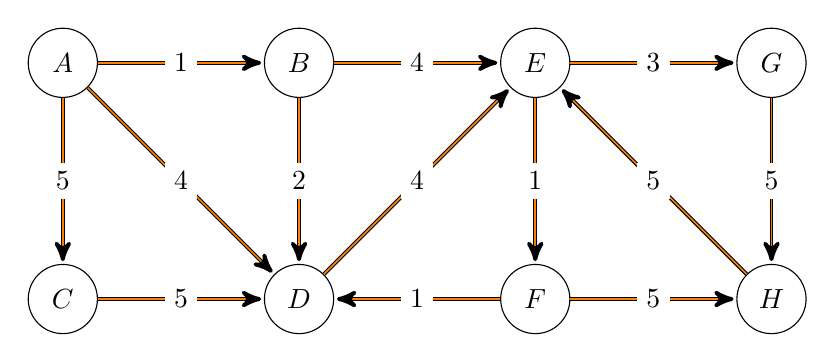
\begin{tikzpicture}[>=stealth',shorten >=1pt,node distance=3cm,on grid,initial/.style    ={}]
  \node[state]          (A)                        {$A$};
  \node[state]          (B) [right =of A]    {$B$};
  \node[state]          (C) [below =of A]    {$C$};
  \node[state]          (D) [below =of B]    {$D$};
  \node[state]          (E) [right =of B]    {$E$};
  \node[state]          (F) [below =of E]    {$F$};
  \node[state]          (G) [right =of E]    {$G$};
  \node[state]          (H) [right =of F]    {$H$};

\tikzset{mystyle/.style={->,double=orange}} 
\tikzset{every node/.style={fill=white}} 
\path (A)     edge [mystyle]    node   {$1$} (B)
      (A)     edge [mystyle]    node   {$5$} (C)
      (A)     edge [mystyle]    node   {$4$} (D)
      (B)     edge [mystyle]    node   {$2$} (D)
      (B)     edge [mystyle]    node   {$4$} (E)
      (D)     edge [mystyle]   node   {$4$} (E)
      (C)     edge [mystyle]   node   {$5$} (D) 
      (E)     edge [mystyle]   node   {$3$} (G)
      (E)     edge [mystyle]   node   {$1$} (F)
      (F)     edge [mystyle]   node   {$5$} (H)
      (F)     edge [mystyle]   node   {$1$} (D)
      (G)     edge [mystyle]   node   {$5$} (H)
      (H)     edge [mystyle]   node   {$5$} (E);

\end{tikzpicture}\\

% Bucky
\q{10}{}
There is a country of $n$ islands. $m$ bridges are installed between some of
these islands allowing us to travel in both directions.  We have two factories
on distinct islands and need to transport goods between theses two factories.
However, since each bridge has a weight limit, if an amount of goods exceeding
the weight limit passes though the bridge, the bridge will collapse. We know
that the weight limit of each bridge is at most $w$; you may assume that $w$ is an integer.
Design an algorithm to
find the maximum weight of the goods that can be moved in one transportation.
The time complexity of your algorithm should be $O((n + m) \log w)$. You can
get partial credits if you design an algorithm of $O((n + m)w)$.

% Bucky
\q{10}{}
For a given directed graph $G = (V, E)$, let us denote $V = \{1, 2, ..., n\}$.
Define a function $D(G, s, t)$ that gives the distance from $s$ to $t$.
%using Dijkstra's algorithm. %Suppose we now are interested in a shortest path from $1$ to $n$.

\begin{enumerate}
    \item We want to get the length of the shortest path from $1$ to $n$ that must pass through a vertex $v$. 
	Prove that $D(G, 1, v) + D(G, v, n)$ gives the desired quantity. You may use proof by contradiction.
    \item We want to get the length of the shortest path from $1$ to $n$ that must pass through two vertices $v$ and $w$. 
	Using the above, find a formula to represent the quantity in terms of the function $D$ and vertices $1, n, v, w$.
\end{enumerate}

%Qimin
%\q{0}{} For a given unsorted array $A = \{a_1, a_2, a_3,...,a_n\}$ with $n$ distinct numbers, please design an $O(nlogn)$ time algorithm to find the smallest 30\% elements in $A$ without sorting the entire $A$ (if the size $n$ is 10, find the largest 3 elements; if the size $n$ is 15, find the largest 4 elements). \emph{Hint: priority queue and its size.}

% Tianyang
\q{8}{} You are given a directed graph $G = (V,E)$ and a vertex $s\in V$. Each edge $e$ is assigned with a length $l(e)$, possibly with negative value. We know that there is no negative cycle in this graph, and that the only negative edges are the ones that leave the vertex $s$. That is, $l(s, v) < 0$ for all $(s, v) \in E$, and $l(u,v) > 0$ for all $u\neq s$ and $(u,v)\in E$. If we run Dijkstra’s algorithm starting at $s$, will it fail on this graph? Prove your conclusion.


\end{qunlist}
\end{document}
